\subsection{Slučaj upotrebe: Upravljanje verzijama scenarija}

\subsubsection*{Kratak opis}

Scenarista kreira scenario za animirani film i razrađuje ga u scene, čime
nastaje prva verzija scenarija. Svaka naredna izmena čuva se kao nova verzija,
a scenarista može da pregleda i poredi verzije i da se vrati na neku od
prethodnih. Verzija se šalje reditelju na odobravanje.

\subsubsection*{Akteri}
\begin{itemize}
    \item \textbf{Scenarista} -- kreira scenario, razrađuje ga u scene i upravlja njegovim verzijama.
    \item \textbf{Reditelj} -- pregleda poslatu verziju scenarija i odobrava je ili vraća na doradu.
\end{itemize}

\subsubsection*{Preduslovi}
\begin{itemize}
    \item Scenarista je prijavljen na sistem i angažovan na projektu.
    \item Projekat animiranog filma postoji u sistemu.
\end{itemize}

\subsubsection*{Postuslovi}
\begin{itemize}
    \item Scenario je sačuvan u sistemu, a svaka izmena je zabeležena kao zasebna verzija sa autorom, datumom i napomenom.
    \item Ako je verzija poslata na odobravanje, reditelj je obavešten.
\end{itemize}

\subsubsection*{Osnovni tok}
\begin{enumerate}
    \item Scenarista bira projekat i opciju ,,Kreiraj scenario''.
    \item Sistem prikazuje formu za unos osnovnih podataka: naslov, žanr, kratak sinopsis i ciljno trajanje filma.
    \item Scenarista popunjava formu i potvrđuje unos.
    \item Sistem proverava podatke i čuva scenario kao verziju 1 sa statusom ,,U izradi''.
    \item Scenarista bira opciju ,,Dodaj scenu'' i unosi podatke o sceni: redni broj, naziv, opis radnje, lokaciju, likove, dijaloge i okvirno trajanje.
    \item Sistem proverava podatke i dodaje scenu u aktuelnu verziju. Koraci 5 i 6 se ponavljaju dok scenarista ne unese sve scene.
    \item Scenarista bira opciju ,,Pošalji na odobravanje''.
    \item Sistem menja status verzije u ,,Poslata na odobravanje'', obaveštava reditelja i prikazuje poruku o uspešnom slanju.
\end{enumerate}

\subsubsection*{Podtokovi}

\paragraph*{P1: Kreiranje nove verzije}
\begin{enumerate}
    \item Scenarista na stranici scenarija bira opciju ,,Izmeni scenario''.
    \item Sistem prikazuje aktuelnu verziju za izmenu, a scenarista menja podatke scenarija i/ili dodaje, menja i briše scene.
    \item Scenarista bira opciju ,,Sačuvaj kao novu verziju'' i unosi napomenu o izmenama.
    \item Sistem čuva novu verziju sa sledećim rednim brojem i postavlja je kao aktuelnu. Prethodna verzija ostaje nepromenjena.
\end{enumerate}

\paragraph*{P2: Pregled i poređenje verzija}
\begin{enumerate}
    \item Scenarista bira opciju ,,Istorija verzija''.
    \item Sistem prikazuje listu svih verzija: redni broj, autor, datum, napomena i status.
    \item Scenarista bira jednu verziju za pregled ili dve verzije za poređenje.
    \item Sistem prikazuje sadržaj izabrane verzije samo za čitanje, odnosno razlike između dve izabrane verzije (dodate, izmenjene i obrisane scene).
\end{enumerate}

\paragraph*{P3: Vraćanje na prethodnu verziju}
\begin{enumerate}
    \item U istoriji verzija scenarista bira stariju verziju i opciju ,,Vrati na ovu verziju''.
    \item Sistem traži potvrdu, a scenarista potvrđuje.
    \item Sistem pravi novu verziju sa sadržajem izabrane starije verzije i postavlja je kao aktuelnu. Sve verzije ostaju sačuvane.
\end{enumerate}

\subsubsection*{Alternativni tokovi}

\paragraph*{A1: Nepopunjena obavezna polja}
\begin{itemize}
    \item U koracima 4 i 6 osnovnog toka, kao i u koraku 4 podtoka P1, ako neko obavezno polje nije popunjeno, sistem ga označava i vraća scenaristu na unos.
\end{itemize}

\paragraph*{A2: Scenario već postoji}
\begin{itemize}
    \item U koraku 1 osnovnog toka, ako projekat već ima scenario, sistem ne dozvoljava kreiranje novog, već nudi izmenu postojećeg (podtok P1).
\end{itemize}

\paragraph*{A3: Nema izmena}
\begin{itemize}
    \item U koraku 3 podtoka P1, ako nijedna izmena nije napravljena, sistem ne pravi novu verziju i obaveštava scenaristu.
\end{itemize}

\paragraph*{A4: Odustajanje}
\begin{itemize}
    \item U bilo kom koraku scenarista može da odustane; sistem ne čuva nesačuvane izmene i vraća ga na stranicu projekta.
\end{itemize}

\subsubsection*{Specijalni zahtevi}
\begin{itemize}
    \item Sačuvane verzije se nikada ne brišu niti menjaju; istorija je trajna.
    \item Scene koje su već povezane sa storyboardom, animacijom ili zvukom ne smeju se obrisati bez upozorenja.
\end{itemize}

\subsubsection*{Dodatne informacije}
\begin{itemize}
    \item Odobravanje ili vraćanje verzije na doradu od strane reditelja je zaseban slučaj upotrebe.
\end{itemize}


\begin{figure}[H]
	\centering
	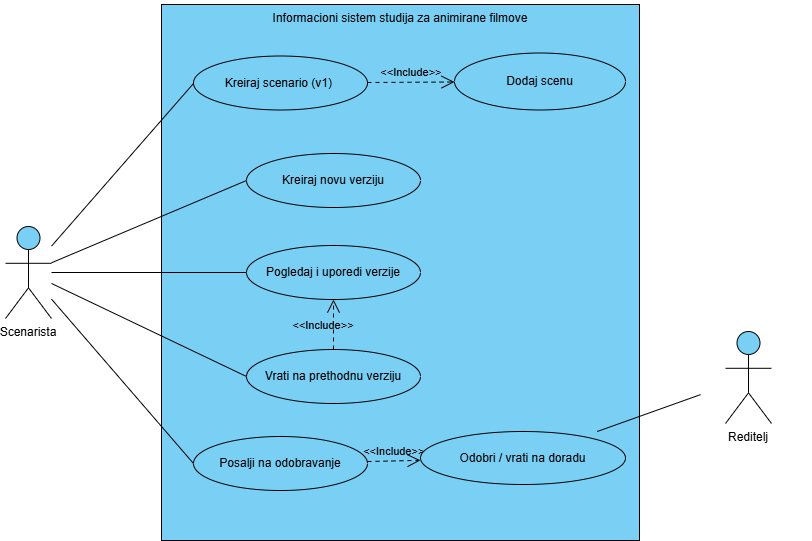
\includegraphics[width=\textwidth]{./dijagrami/dijagrami_slucajeva_upotrebe/upravljanje_verzijama_scenarija.png}
	\caption{Dijagram slučaja upotrebe ,,Upravljanje verzijama scenarija''}
 \end{figure}

\begin{figure}[H]
	\centering
	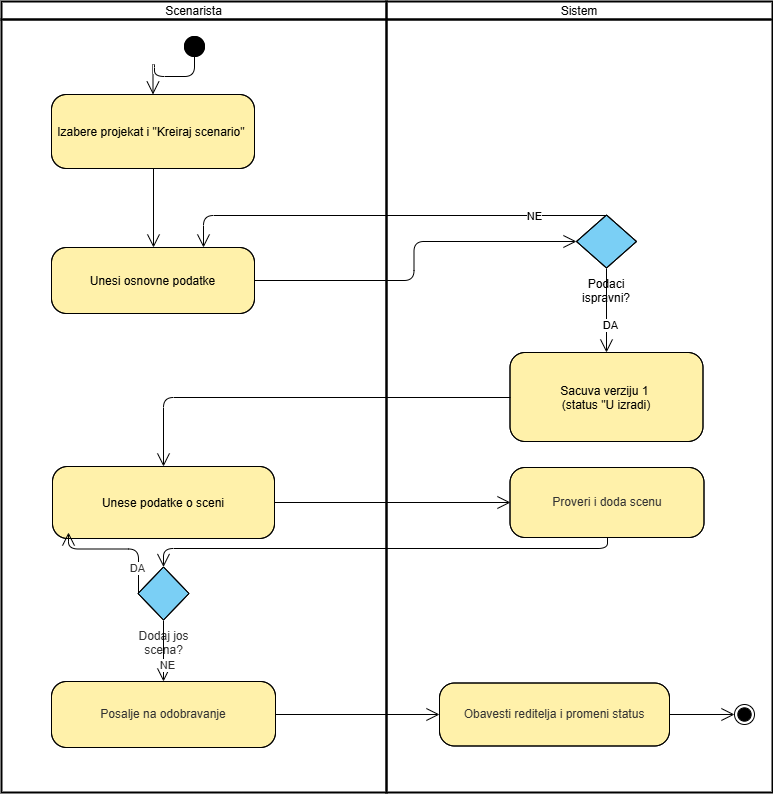
\includegraphics[width=\textwidth]{./dijagrami/dijagrami_aktivnosti/upravljanje_verzijama_scenarija.png}
	\caption{Dijagram aktivnosti ,,Upravljanje verzijama scenarija''}
 \end{figure}

\begin{figure}[H]
	\centering
	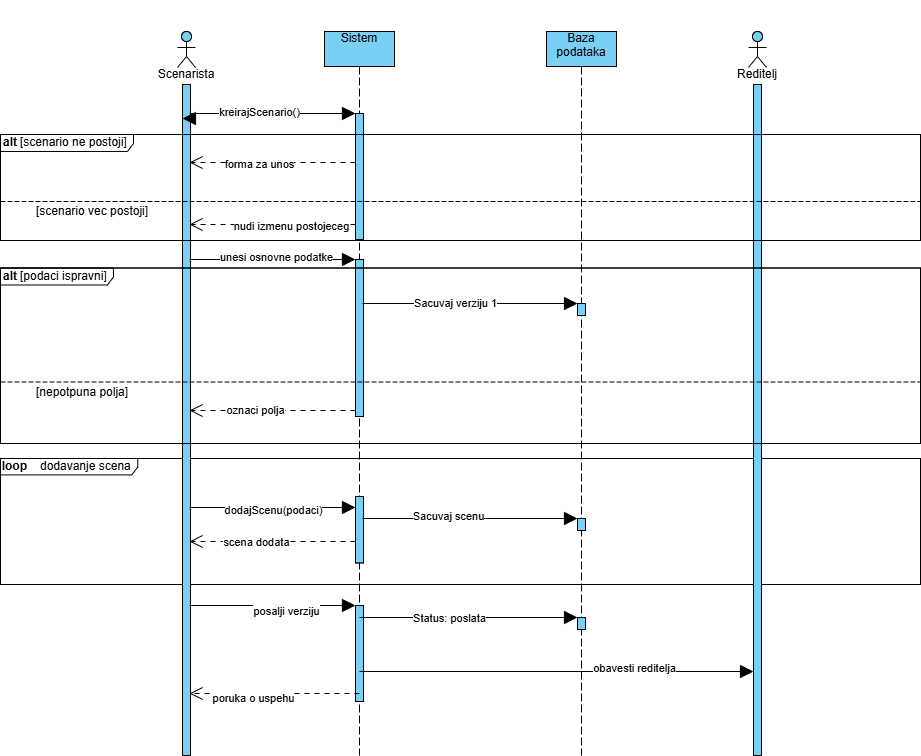
\includegraphics[width=\textwidth]{./dijagrami/dijagrami_sekvence/upravljanje_verzijama_scenarija.png}
	\caption{Dijagram sekvence ,,Upravljanje verzijama scenarija''}
 \end{figure}

\newpage